\section{WiFi-Modul}\label{Appendix:ESP_32}

%\subsection{Tabellarischer Vergleich zwischen ESP32 und ESP8266}\label{Appendix:ESP32_vs_ESP8266}
%
%\begin{table}[H]
%\center
%\begin{tabular}{|l|c|c|}
%\hline
%\textbf{MCU}                    & \textbf{Xtensa Single-Core} & \textbf{Xtensa Dual-Core} \\
%
%			                   & \textbf{32-bit L106 (ESP8266)} & \textbf{32-bit LX6 (ESP32)} \\ \hline
%
%802.11 b/g/n     		& HT20                           & HT40                                       \\
%Bluetooth              	& No                             & Bluetooth 4.2 and BLE                      \\
%Arbeitsfrequenz			& 80 MHz                         & 160 MHz                                    \\
%SRAM                   	& No                             & Yes                                         \\
%Flash                  	& No                             & Yes                                          \\
%GPIO                   	& 17                             & 36                                         \\
%SPI/I2C/I2S/UART       	& 2/1/2/2                        & 4/2/2/2                                    \\
%ADC                    	& 10-bit                         & 12-bit                                     \\
%Ethernet Interface 		& No                             & Yes                                          \\
%Touchsensor           	& No                             & Yes                                          \\
%Temperatursensor     	& No                             & Yes                                          \\
%Hall-Sensor     			& No                             & Yes \\
%Arbeitstemperatur    	& -40ºC to 125ºC                 & -40ºC to 125ºC                             \\
%Price                  	& \$ (3\$ - \$6)                 & \$\$ (\$6 - \$12)    \\                         
%\hline
%\end{tabular}
%\caption{Vergleich ESP8266 zu ESP32. \cite{iainandrew_esp8266_2018}}
%\label{tab:ESP}
%\end{table}

%\subsection{Strapping-Pins}\label{Appendix:ESP32_Strapping}
%
%\begin{table}[H]
%\center
%\begin{tabular}{|c|c|c|c|c|c|c|}
%\hline
%\multicolumn{7}{|c|}{\textbf{Ausgangsspannung internen Spannungsregler (VDD\_SDIO)}}\\
%\hline
%RS232 & ESP & default & \multicolumn{2}{|c|}{\textbf{3.3V}} & \multicolumn{2}{|c|}{\textbf{1.8V}}\\
%\hline
%\sout{RTS} & \sout{IO12} & Pull-down & \multicolumn{2}{|c|}{\sout{\textcolor{red}{0}}\footnotemark} & \multicolumn{2}{|c|}{\sout{1}}\\
%\hline
%\multicolumn{7}{|c|}{\textbf{Boot-Modus}}\\
%\hline
%RS232 & ESP & default & \multicolumn{2}{|c|}{\textbf{SPI-flash Boot}} & \multicolumn{2}{|c|}{\textbf{Download Boot}}\\
%\hline
%DTR & IO0 & Pull-up & \multicolumn{2}{|c|}{1} & \multicolumn{2}{|c|}{0}\\
%\hline
%- & IO2 & Pull-down & \multicolumn{2}{|c|}{Egal} & \multicolumn{2}{|c|}{0}\\
%\hline
%\multicolumn{7}{|c|}{\textbf{Debugging Log Print über U0TXD während Booten}}\\
%\hline
%RS232 & ESP & default & \multicolumn{2}{|c|}{\textbf{U0TXD Active}} & \multicolumn{2}{|c|}{\textbf{U0TXD Silent}}\\
%\hline
%RTS & IO12 & Pull-down & \multicolumn{2}{|c|}{\textcolor{red}{1}} & \multicolumn{2}{|c|}{0}\\
%\hline
%\multicolumn{7}{|c|}{\textbf{Timing\footnotemark des SDIO}}\\
%\hline
%RS232 & ESP & default & \shortstack{FF Sampling \\ FF Output} & \shortstack{FF Sampling \\ SF Output} & \shortstack{SF Sampling \\ FF Output} & \shortstack{SF Sampling \\ SF Output} \\
%\hline
%CTS & IO15 & Pull-up & 0 & 0 & 1 & 1 \\
%\hline
%- & GPIO5 & Pull-up & 0 & 1 & 0 & 1 \\
%\hline
%\end{tabular}
%\caption{Tabelle Pinkonfiguration für Strapping-Pins.\cite[S.13]{espressif_systems_esp32_2020}}
%\label{tab:Strapping_pins}
%\end{table}
%
%\textbf{Spannung des internen Spannungsgeglers (VDD\_SDIO)}
%
%Das WiFi-Modul hat einen eingebauten host controller für SD/SDIO/MMC-Speichergeräte. Dieser kann mit 3.3V (IO12 = 0) oder 1.8V (IO12 = 1) betrieben werden. Wird der Pin auf 1 gesetzt, könnte ein Brown-out der IO-Versorgungspannung VCC\_IO ausgelöst werden.
%
%\textbf{Booting Mode}
%
%Der Pin IO0 gibt vor, ob das WiFi-Modul vom internen SPI-flash bootet (IO0 = 1) oder ob neuer Code in den flash Speicher geschrieben wird (IO0 = 0). Soll das WiFi-Modul vom Flash-Speicher booten, so hat der Pin IO2 kein Einfluss, um jedoch den Code speichern zu können, muss der Pin auf 0 sein.
%
%\textbf{De-/Aktivieren vom Debug-Log über U0TXD während dem Bootvorgang}
%
%Über den Pin IO12 kann konfiguriert werden, ob während dem Booten ein Debug-Log über die Serielleschnittstelle gesendet wird (IO12 = 1) oder nicht (IO12 = 0).
%
%\textbf{Timing der Kommunikation mit dem SDIO Slave}:
%
%Über die Pins IO15 und IO5 kann das Übertragungsprotokoll des SDIO-Slaves festgelegt werden. Dabei kommt es darauf an, ob das Sampling auf eine fallende Flanke (IO15 = 0) oder steigende Flanke (IO15 = 1) geschehen soll, und ob der Output auf eine fallende Flanke (IO5 = 0) oder steigende Flanke (IO5 = 1) geschehen soll.
%
%\cite{espressif_systems_esp32_2020} \cite{various_contributors_espressifesptool_2020}
%
%\footnotetext[18]{Da das ESP32-WROOM-32U einen 3.3V SPI flash integriert hat, kann der MTDI nicht auf 1 gesetzt werden, wenn die Module aufgestartet sind.}
%\footnotetext{FF = Fallende Flanke, SF = Steigende Flanke}

\subsection{Inbetriebnahme}

\subsubsection{Arduino IDE}\label{Appendix:ESP32_Arduino_IDE}
%
%\begin{figure}[H]
%	\centering
%	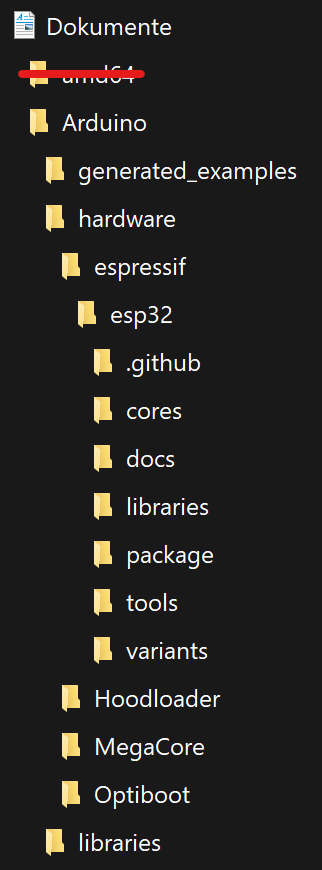
\includegraphics[width=0.2\textwidth]{graphics/ESP32_Ordner}
%	\caption{Ordnerstruktur Boards Arduino IDE.}
%	\label{fig:ESP32_Ordner}
%\end{figure}

\begin{figure}[H]
	\centering
	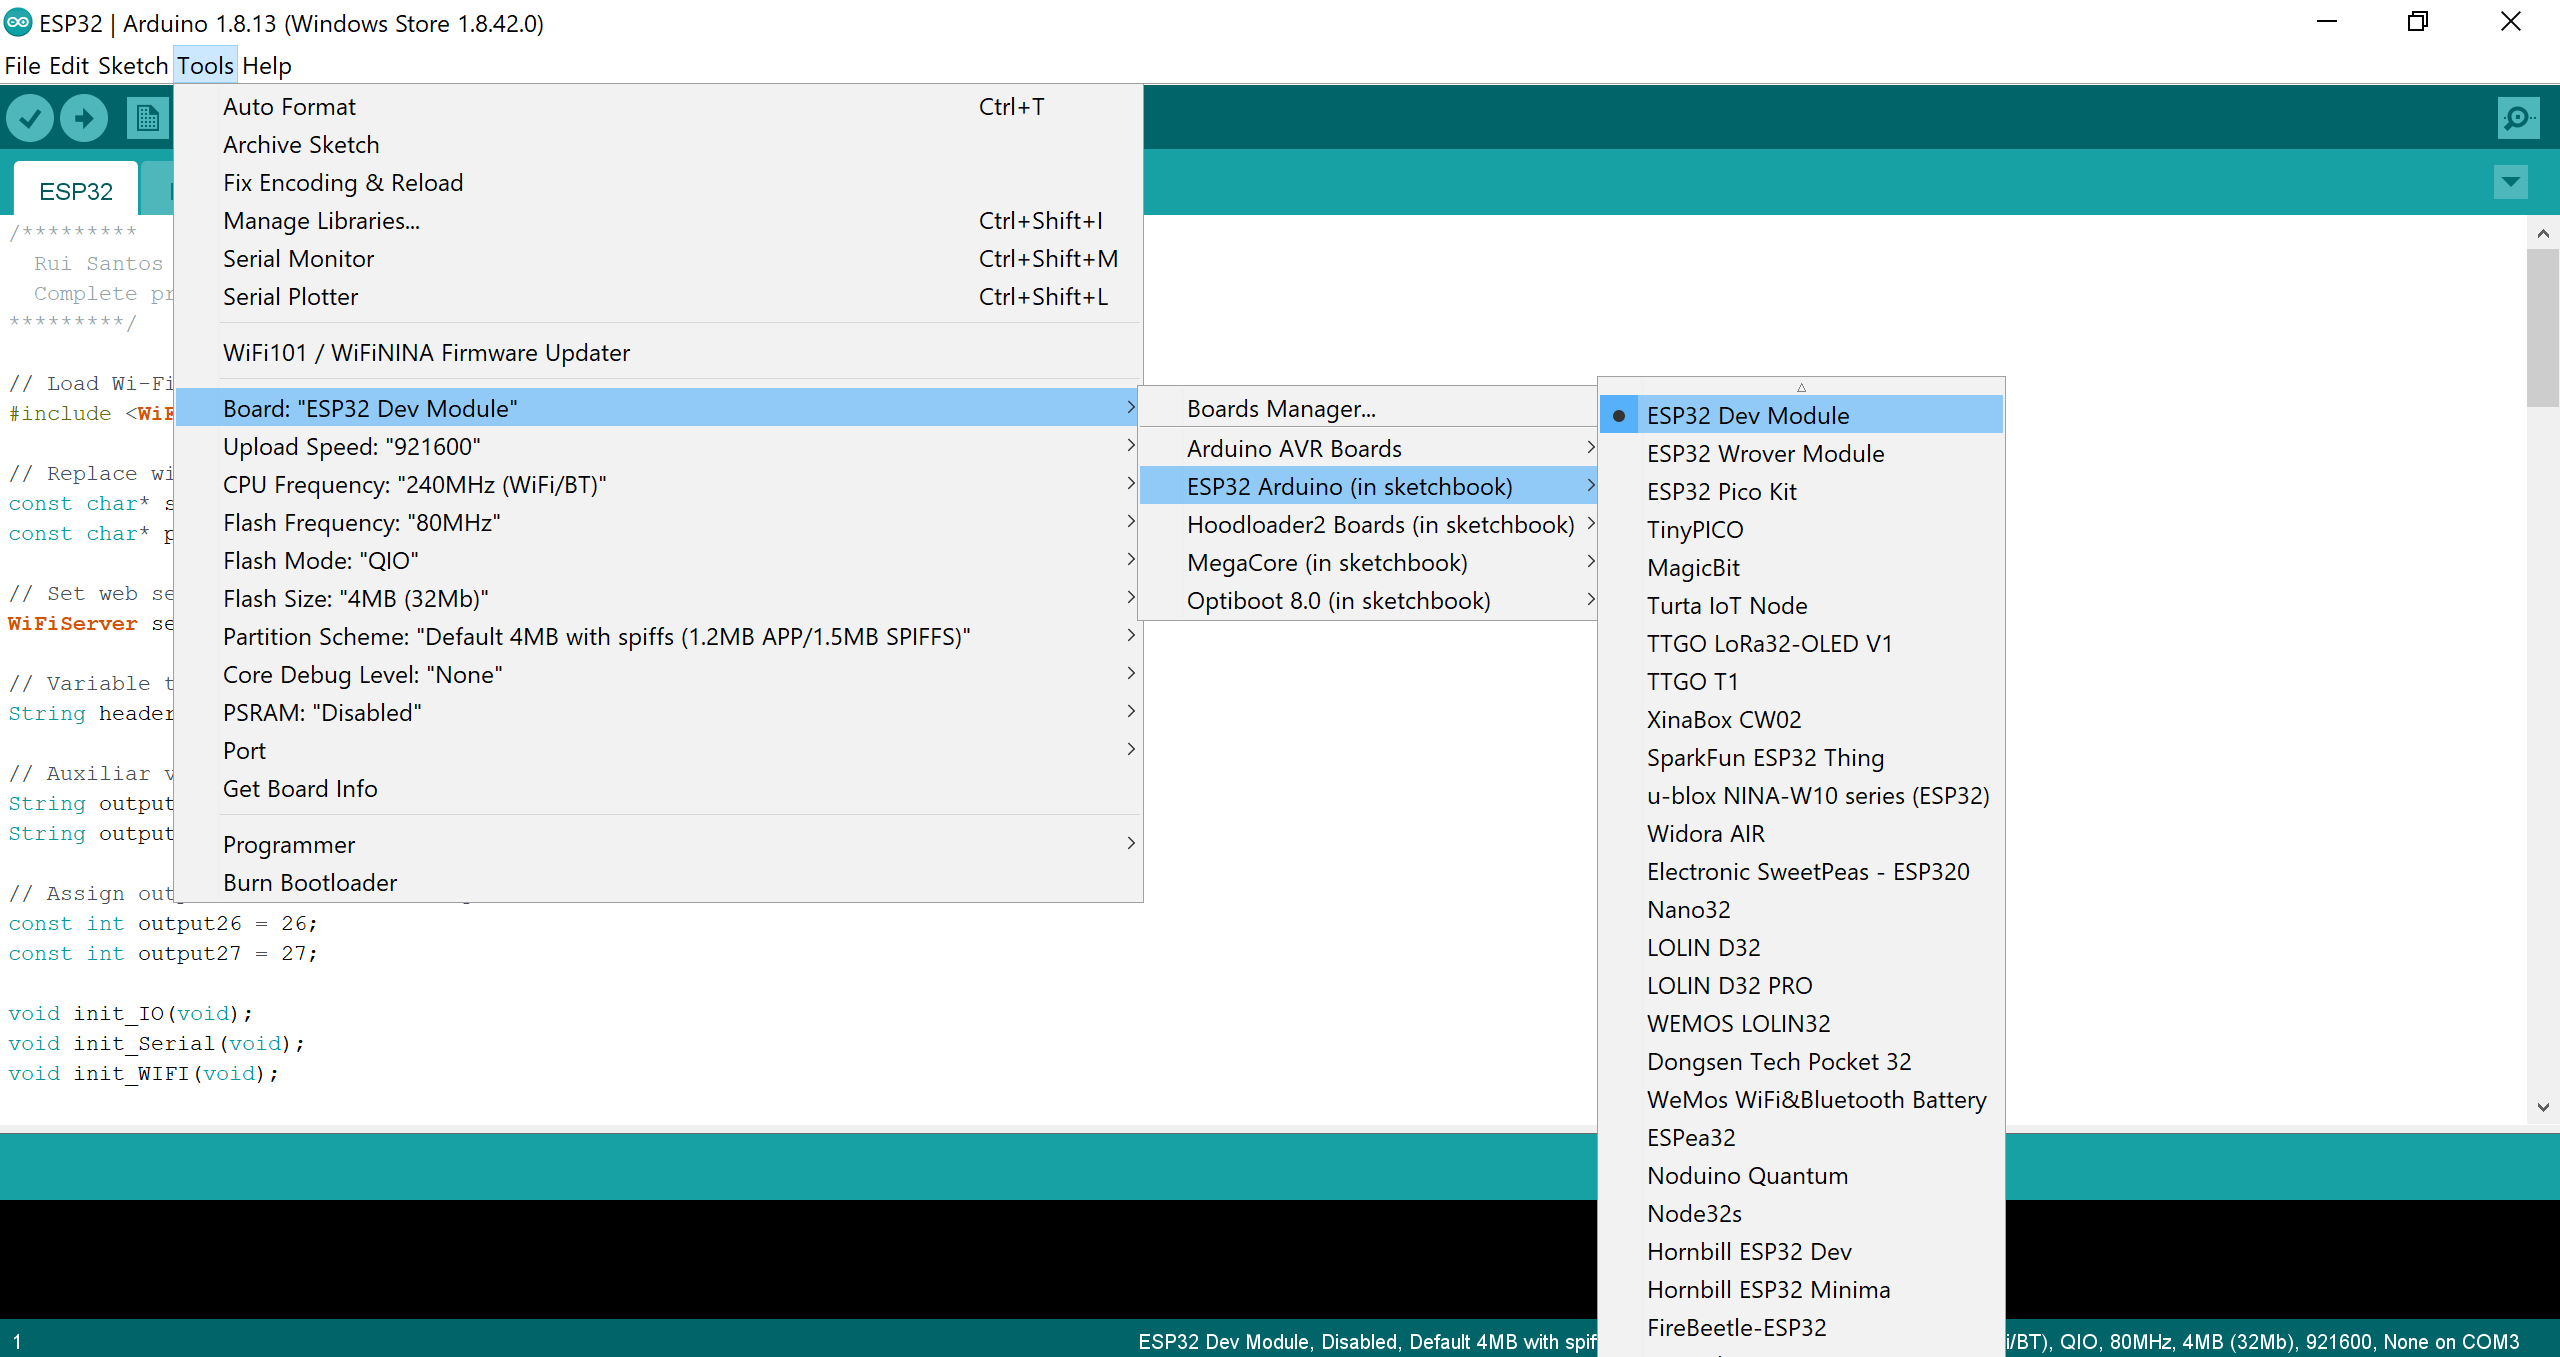
\includegraphics[width=\textwidth]{graphics/ESP32_Arduino_IDE}
	\caption{ESP32 auswählen in der Arduino IDEs.}
	\label{fig:ESP32_Arduino_IDE}
\end{figure}
%
%\begin{figure}[H]
%	\centering
%	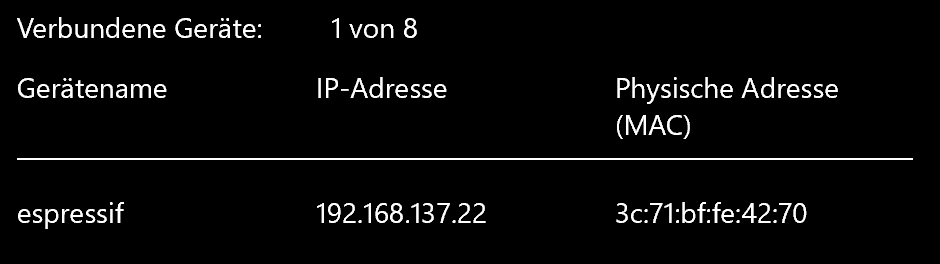
\includegraphics[width=0.7\textwidth]{graphics/ESP32_Verbundene_Geraete}
%	\caption{WiFi-Modul verbindet sich nach Hochladen des Codes mit dem WiFi.}
%	\label{fig:ESP32_Verbundene_Geraete}
%\end{figure}

\begin{figure}[H]
	\centering
	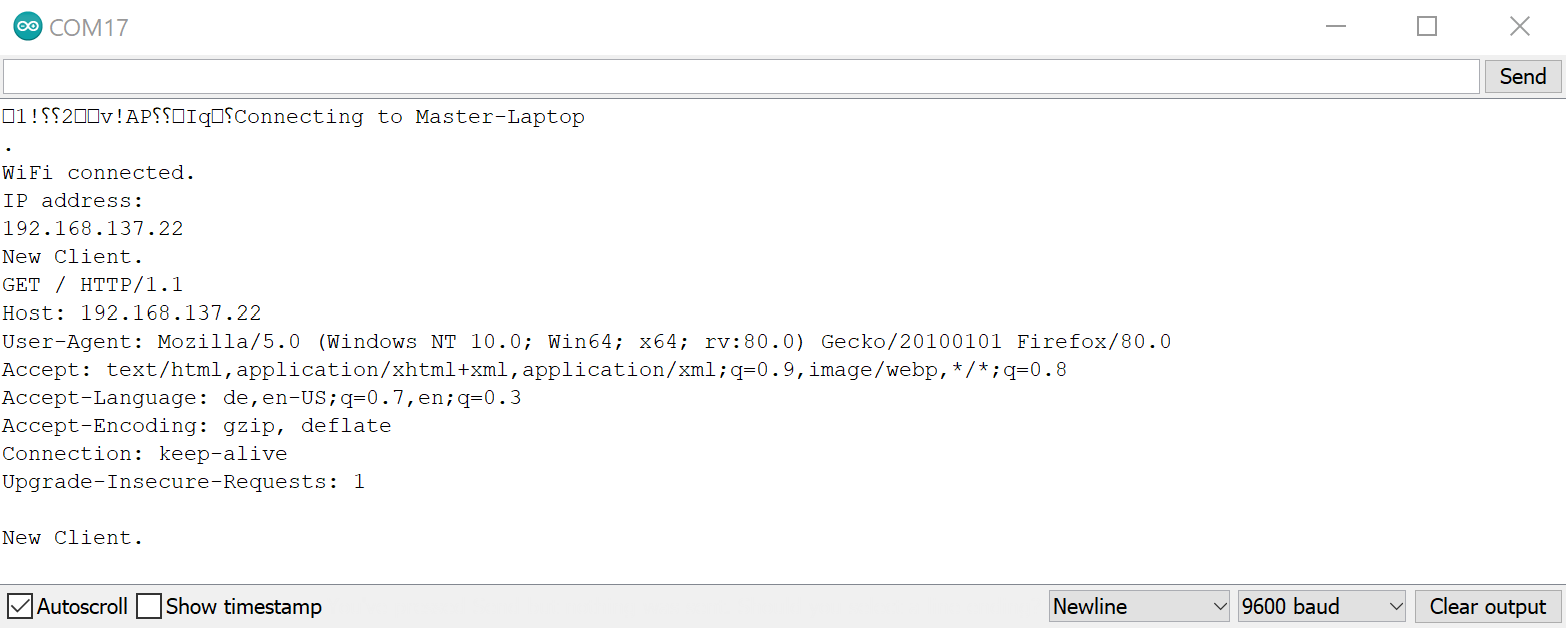
\includegraphics[width=\textwidth]{graphics/ESP32_Serial_Monitor}
	\caption{WiFi-Modul erkennt Netzwerk und Client (Browser).}
	\label{fig:ESP32_Serial_Monitor}
\end{figure}

\begin{figure}[H]
	\centering
	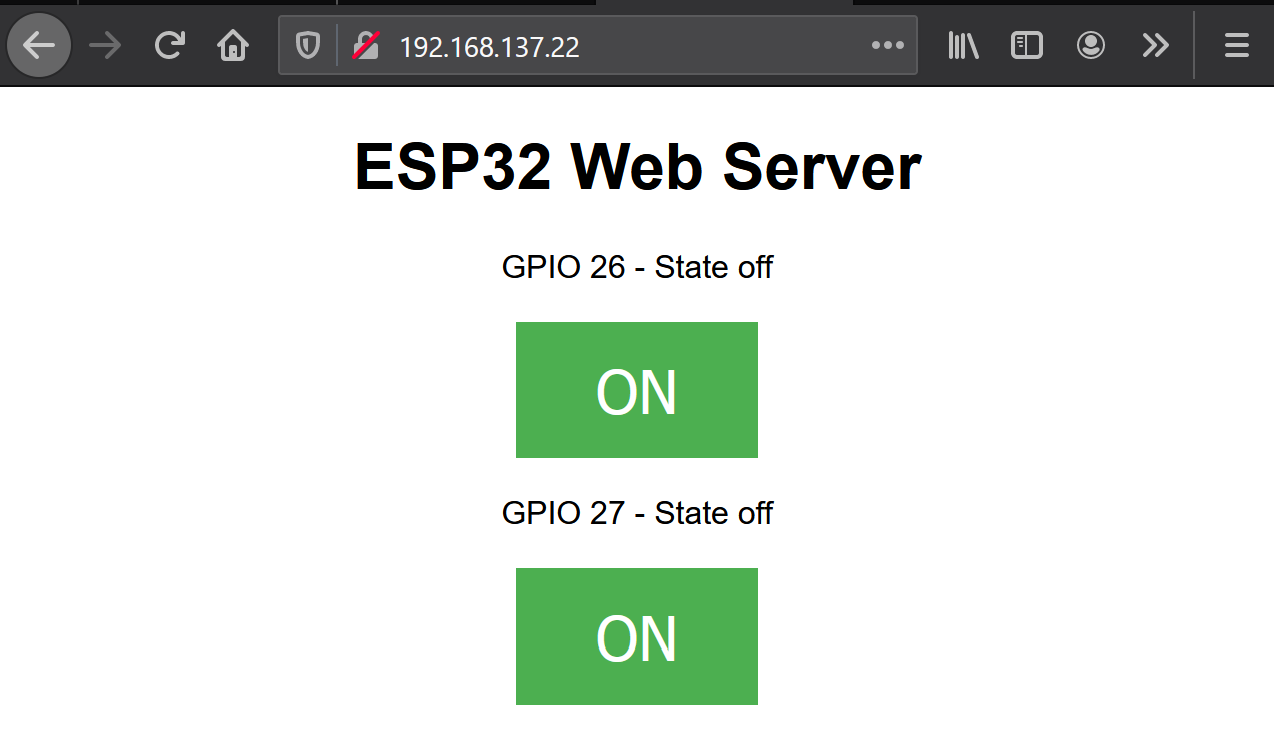
\includegraphics[width=\textwidth]{graphics/ESP32_Webserver}
	\caption{WiFi-Modul als Host (Browseransicht).}
	\label{fig:ESP32_Webserver}
\end{figure}